\begin{solution}{Question 1}\label{ques:1}
    \begin{question}
    Given an alphabet $\Gamma = \{l_1,...,l_k\} $, construct an $NFA$ that accepts strings that don’t have all the characters from $\Gamma$. Can you give an $NFA$ with $k$ states?
    \end{question}
    \tcblower{}
    \begin{proof}[Solution]
    We have to construct an $NFA$ such that the string $(x)$ to be accepted has atmost $k-1$ unique letters used out of language $\Gamma$. The regular expression for the problem can be defined as $x = [\Sigma\setminus l_1]^* + [\Sigma\setminus l_2]^*+ \dots + [\Sigma\setminus l_{k-1}]^*+[\Sigma\setminus l_k]^*$\\
    (where + is a union and we are following code regex syntax)\\
    For every regular expression, we can define an $\epsilon-NFA$. The $NFA (Q, \Sigma, \delta, q_0, F)$ created by aforementioned regular expression is defined by following diagram:
    \begin{center}
        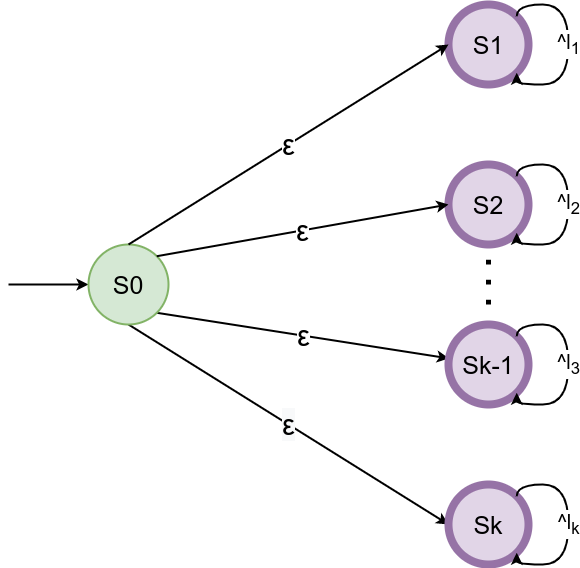
\includegraphics[scale=0.6]{NFA_bigalphabet.png}
    \end{center}
    There are a total of $k+1$ states ($Q = {S0,S1,...SK}$), $\Sigma$ is the alphabet which can be equal to $\Gamma$. The transitions $\delta$ are as shown in the figure. $^\wedge l_r$ denotes all characters allowed for transition except $l_r$ in state $Sr$. $q_0$ is initial state which is $S0$ here. The final states $F$ are all states except $S0$.\\
    We could not give an $NFA$ with $k$ states as the regex couldn't be reduced further nor the $NFA$ since it considers all the $k$ characters apart from the start state involving $\epsilon$ transitions.
    
    \end{proof}
\end{solution}
